\subsubsection*{January 24, 2020}

We can do some fun stuff in Mathematica. (***)

\begin{minted}[linenos=true]{mathematica}
(*Setting a degree n*)
n = 3;
(*Defined Polynomial*)
p[x_] := x^2 + 1;
(*Creating a table from 0 to n-1 (digits in Subscript[Z, n])*)
zn = Table[k, {k, 0, n - 1}];
(*Calcualtes the degree of polynomial p[x]*)
deg = Length[CoefficientList[p[x], x]] - 1;
(*Finds tuples of length deg with elements from zn*)
Tuples[zn, deg];
(*Turns a Tuple to a polynomial*)
tuple2poly[t_] := Module[{},
  l = Length[t];
  Return[Sum[t[[i]] x^(i - 1), {i, 1, l}]]
  ]
  (*Polynomial form of tuples*)
polys = 
 Sort[Map[tuple2poly, Tuples[zn, deg]]]
\end{minted}
\includegraphics{notebooks/quotientrings/gr7.eps}
\begin{minted}[linenos=true]{mathematica}
	add = Table[
   PolynomialMod[
    PolynomialRemainder[polys[[i]] + polys[[j]], p[x], x], n], {i, 1, 
    Length[polys]}, {j, 1, Length[polys]}];
TableForm[add, TableHeadings -> {polys, polys}]
\end{minted}
\includegraphics[width=\textwidth]{notebooks/quotientrings/gr9.eps}
\begin{minted}[linenos=true]{mathematica}
polys1 = DeleteCases[polys, 0]
mult = Table[
   PolynomialMod[
    PolynomialRemainder[polys1[[i]]*polys1[[j]], p[x], x], n], {i, 1, 
    Length[polys1]}, {j, 1, Length[polys1]}];
TableForm[mult, TableHeadings -> {polys1, polys1}]
\end{minted}
\includegraphics{notebooks/quotientrings/gr11.eps} \\

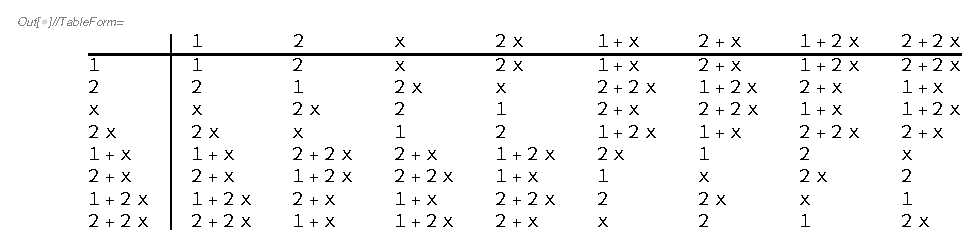
\includegraphics[width=\textwidth]{notebooks/quotientrings/gr12.eps}

\begin{proposition}
	A commutative ring with identity $R$ that does not have any proper ideals is a field. 
\end{proposition}
\begin{proof}
	We show that every element in $R$ is a unit. 
	
	Consider $I=aR$. Since $R$ only has trivial ideals, $aR=R$. Since $1\in R$, there exists a solution to $ax=1$, so $a$ is a unit. 
\end{proof}
